\documentclass[12pt,a4paper]{article}
\usepackage[portuguese]{babel}
\usepackage[a4paper]{geometry}
\usepackage[utf8]{inputenc}
\usepackage{lmodern}      % letra, símbolos, etc.
\usepackage{cmap}
\usepackage{setspace} % Espaçamento entre linhas 
\usepackage{microtype} % espaçamento entre letras e palavras, colocar depois da fonte
\usepackage{siunitx} % unidade si 
\sisetup{output-decimal-marker = {,}}
\usepackage[version=4]{mhchem}
\usepackage{caption} % caption
\usepackage{subcaption} % caption   
\usepackage{graphicx}     % gráficos
\usepackage{tabularx}     % tabelas
\usepackage{booktabs}  
\usepackage[table]{xcolor} % cores
\usepackage{multirow}
\usepackage{makeidx}
\usepackage{ragged2e}
\addto\captionsportuguese{\renewcommand{\refname}{Referências}}
\usepackage[colorlinks=true,citecolor=black,linkcolor=black,bookmarks=true]{hyperref}
\usepackage{natbib}
\usepackage{float}
\usepackage{indentfirst}

\onehalfspacing

\begin{document}

\pagenumbering{arabic}

\thispagestyle{empty}
\begin{minipage}{\textwidth}\centering
Universidade de São Paulo \\
Instituto de Ciências Matemáticas e Computação \\
Desenvolvimento de Código Otimizado - SSC 0951 \\
\end{minipage}

\vspace{5cm}

\begin{minipage}{\textwidth}\centering
\Large Relatório Trabalho 3  \\
\vspace{2cm}
\Large \textbf{Otimização do Compilador}
\end{minipage}

\vspace{3cm}

\begin{minipage}{\linewidth}\centering
\begin{enumerate}
     \item Lucas G. Meneses   \space \space \space \space \space \space  Número: 13671615
      \item Henrique S. Marques  \space \space Número: 11815722
      \item Carlos F. C. Lemos  \space \space \space \space Número: 12542630
\end{enumerate}
\end{minipage}

\vfill

\begin{minipage}{\linewidth}
\centering\today, \\
São Carlos, SP, \\
Brasil
\end{minipage}

\clearpage
\thispagestyle{empty}

\tableofcontents

\section{Introdução}

Os compiladores desempenham um papel crucial na tradução do código-fonte de um programa para a linguagem de máquina executável, e ao longo das últimas décadas, têm evoluído significativamente para incorporar otimizações que melhoram o desempenho e a eficiência dos programas gerados. Entre os compiladores notáveis, destaca-se o GCC (\textit{GNU Compiler Collection}), uma ferramenta de código aberto amplamente utilizada. As otimizações introduzidas por compiladores como o GCC visam aprimorar diversos aspectos do código, desde o uso eficiente dos recursos do processador até a redução do tempo de execução.

Uma das principais áreas de otimização reside na melhoria da eficiência do código gerado, buscando reduzir o número de instruções executadas sem comprometer a semântica do programa. O GCC utiliza uma variedade de técnicas, como \textit{inlining} de funções, eliminação de código morto e propagação de constantes, para transformar o código-fonte em uma forma mais eficiente. Essas otimizações não apenas resultam em programas mais rápidos, mas também contribuem para a economia de recursos computacionais.

Além disso, o GCC incorpora estratégias avançadas de otimização durante a compilação, como a vetorização de \textit{loops} e o agendamento de instruções, que exploram as capacidades específicas do \textit{hardware} de destino. Isso permite que o compilador adapte o código gerado às características da arquitetura subjacente, tirando proveito de recursos, como \textit{pipelines} de instruções e unidades de execução paralela. Neste trabalho em específico, o objetivo foi a testagem de \textit{flags} de otimização durante a compilação, com o objetivo de avaliar o impacto nas métricas de tempo de execução, tempo de compilação e tamanho do executável para dois programas selecionados do CLBG.

\section{Metodologia} \label{sec:metodologia}

Para a realização de todos os experimentos, foi utilizado um computador rodando o Sistema Operacional Arch Linux, cuja CPU é um AMD Ryzen 7 5700X com frequência de \textit{clock} de \SI{3,4}{\giga\hertz}, 8 núcleos e 16 \textit{threads}. Quanto à memória, o computador faz uso de \SI{32}{\giga\byte} de RAM do tipo DDR4, cache L1 de \SI{512}{\kilo\byte}, L2 de \SI{4}{\mega\byte} e L3 de \SI{32}{\mega\byte}.

Nesse sentido, dois programas do \href{https://benchmarksgame-team.pages.debian.net/benchmarksgame/}{CLBG} (\textit{Computer Language Benchmarks Game}) foram selecionados (nomearemos de \href{https://benchmarksgame-team.pages.debian.net/benchmarksgame/program/pidigits-gcc-1.html}{\textit{code1}} e \href{https://benchmarksgame-team.pages.debian.net/benchmarksgame/program/pidigits-gcc-2.html}{\textit{code2}}) para teste quanto ao tempo de compilação (Seção \ref{sec:tempo_compilacao}), tamanho do executável gerado (Seção \ref{sec:tamanho_executavel}) e tempo de execução (Seção \ref{sec:tempo_execucao}). Tais códigos referem-se a dois modos diferentes de se calcular casas decimais do número pi ($\pi$), sendo adequados para testes de \textit{benchmark}. Dessa maneira, foram compilados e executados 10 vezes, computamos a média aritmética e intervalo de confiança de cada métrica avaliada, para cada uma das seguintes \textit{flags} de compilação:

\begin{itemize}
    \item \textbf{O0} (sem otimizações): nenhuma otimização é ativada.
    \item \textbf{O1} (otimização leve): aplica otimizações que não aumentam significativamente o tempo de compilação, focadas em melhorar o desempenho sem comprometer muito o tempo de compilação.
    \item \textbf{O2} (otimização moderada): introduz otimizações adicionais, incluindo \textit{inlining} de funções e reordenação de código, proporcionando melhorias substanciais no desempenho, mas com um aumento modesto no tempo de compilação.
    \item \textbf{O3} (otimização agressiva): aplica otimizações mais agressivas, como vetorização de \textit{loops} e \textit{inlining} mais agressivo, para maximizar o desempenho, embora isso possa aumentar significativamente o tempo de compilação.
    \item \textbf{Os} (otimização de tamanho): foca na redução do tamanho do executável, sacrificando potencialmente o desempenho. Isso é útil quando o tamanho do arquivo executável é crítico, por exemplo, em ambientes com restrições de armazenamento.
\end{itemize}

\section{Resultados}

\subsection{Tempo de Compilação} \label{sec:tempo_compilacao}

A Figura \ref{fig:tempo_compilacao} sumariza os resultados obtidos em relação ao tempo de compilação, variando a \textit{flag} de otimização utilizada.

\begin{figure}[H]
\centering
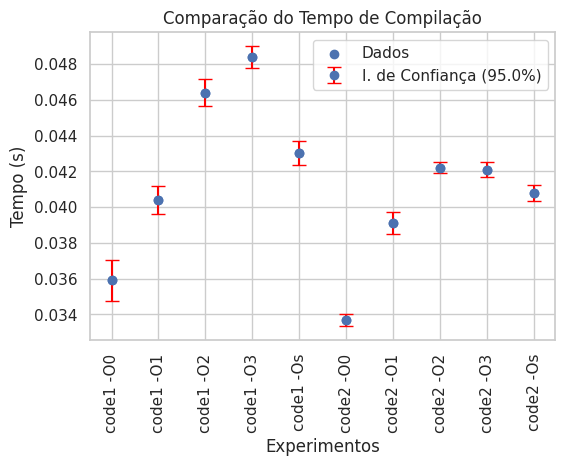
\includegraphics[width=0.80\linewidth]{Figures/comparacao_compilacao_codigo_intervalo.png}
\caption{Tempos de compilação (\si{\second}) em função dos códigos e das \textit{flags} de otimização utilizadas. Os círculos azuis indicam a média dos dados obtidos para cada experimento e as barras vermelhas mostram o intervalo de confiança de \SI{95}{\percent}.}
\label{fig:tempo_compilacao}
\end{figure}

Conforme esperado, os programas tiveram seu tempo de compilação aumentados ao se intensificar o nível de otimização exigido pelo compilador, em especial o \textit{code1}, cujo aumento foi mais significativo. No caso do \textit{code2}, pode-se verificar que os tempos de compilação com as \textit{flags} O2 e O3 foram estatísticamente equivalentes, apesar de maiores quando comparados às \textit{flags} O0 e O1. Quanto à otimização de tamanho de executável (\textit{flag} Os), obteve-se um tempo de compilação intermediário (entre O1 e O2) para ambos os programas. 

\subsection{Tamanho do Executável} \label{sec:tamanho_executavel}

A Figura \ref{fig:tamanho_executavel} sumariza os resultados obtidos em relação ao tamanho do executável gerado, variando a \textit{flag} de otimização utilizada.

\begin{figure}[H]
\centering
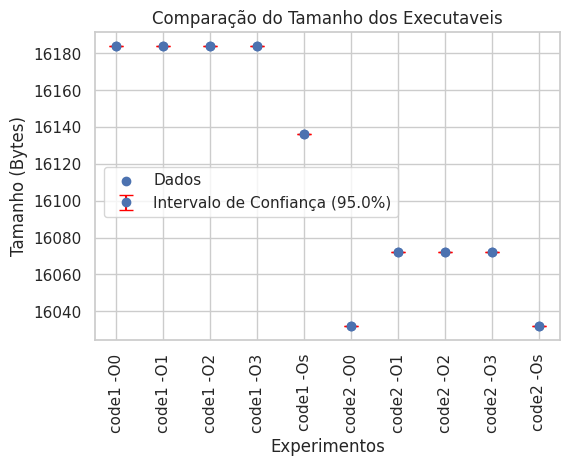
\includegraphics[width=0.80\linewidth]{Figures/comparacao_tamanho_codigo_intervalo.png}
\caption{Tamanho dos executáveis gerados (\si{\kilo\byte}) em função dos códigos e das \textit{flags} de otimização utilizadas. Os círculos azuis indicam a média dos dados obtidos para cada experimento e as barras vermelhas mostram o intervalo de confiança de \SI{95}{\percent}.}
\label{fig:tamanho_executavel}
\end{figure}

Em relação a esta métrica, as \textit{flags} referentes à otimização de desempenho (O1, O2 e O3) não alteraram o tamanho dos executáveis em ambos os programas (aproximadamente \SI{16,18}{\kilo\byte} para \textit{code1} e \SI{16,07}{\kilo\byte} para \textit{code2}). Entretanto, tais \textit{flags} geraram executáveis maiores para o \textit{code2} quando comparadas à \textit{flag} O0, correspondente à nenhuma otimização, situação não verificada para \textit{code1}, com mesmo tamanho de executável para as 4 \textit{flags}. Por outro lado, a \textit{flag} Os teve sucesso na redução do tamanho do executável para os programas, gerando os menores executáveis entre os experimentos (tamanho estatísticamente "empatado" com O0, no \textit{code2}). 

\subsection{Tempo de Execução} \label{sec:tempo_execucao}

A Figura \ref{fig:tempo_execucao} sumariza os resultados obtidos em relação ao tempo de execução dos programas selecionados, variando a \textit{flag} de otimização utilizada.

\begin{figure}[H]
\centering
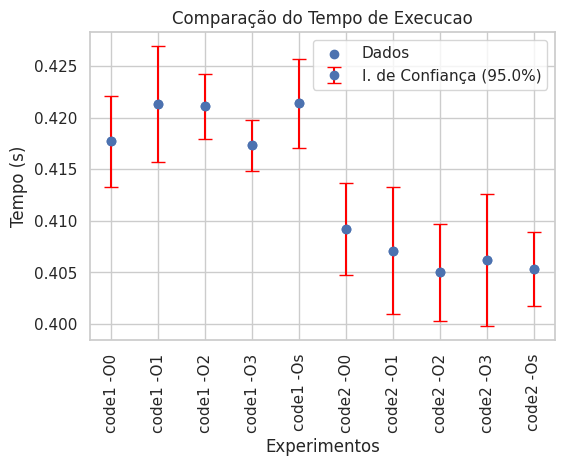
\includegraphics[width=0.80\linewidth]{Figures/comparacao_execucao_codigo_intervalo.png}
\caption{Tempos de execução (\si{\second}) em função dos códigos e das \textit{flags} de otimização utilizadas. Os círculos azuis indicam a média dos dados obtidos para cada experimento e as barras vermelhas mostram o intervalo de confiança de \SI{95}{\percent}.}
\label{fig:tempo_execucao}
\end{figure}

Ao se avaliar os intervalos de confiança obtidos com a execução repetida de cada um dos códigos, verificou-se que, para a arquitetura utilizada no experimento, as \textit{flags} de otimização do compilador, bem como a \textit{flag} O0 (sem otimização), não alteraram significativamente os tempos de execução de ambos os programas. 

Apesar de contra-intuitivo, tal resultado pode estar relacionados à natureza robusta e eficiente do AMD Ryzen 7 5700X (processador empregado nos experimentos, conforme descrito na Seção \ref{sec:metodologia}) em lidar com uma variedade de cargas de trabalho. Sua arquitetura avançada, com 8 núcleos e 16 \textit{threads}, combinada com caches L1, L2 e L3 generosas, pode mitigar a necessidade de otimizações agressivas. Se o código dos programas não explorar plenamente as capacidades da arquitetura, ou se os ganhos potenciais das otimizações forem ofuscados pela eficiência intrínseca da arquitetura, é possível que tais \textit{flags} não tenham um impacto perceptível nos tempos de execução.

\section{Conclusões}

Os resultados obtidos neste trabalho fornecem \textit{insights} valiosos sobre o impacto das \textit{flags} de otimização do compilador GCC. Observou-se que, em relação ao tempo de compilação, o aumento do nível de otimização resultou em incrementos esperados nos tempos, sendo mais pronunciado para o código \textit{code1}. Entretanto, em termos de tamanho do executável, as \textit{flags} O1, O2 e O3 não influenciaram significativamente ambos os programas, enquanto a \textit{flag} Os demonstrou eficácia na redução do tamanho do executável. Surpreendentemente, no que diz respeito aos tempos de execução, as \textit{flags} de otimização, incluindo a \textit{flag} O0 (sem otimização), não apresentaram alterações expressivas. Este resultado pode ser atribuído à eficiência intrínseca da arquitetura AMD Ryzen 7 5700X, cujas características robustas e avançadas podem reduzir a dependência de otimizações agressivas para alguns tipos de carga de trabalho, evidenciando a complexidade da relação entre otimizações de compilador e arquiteturas específicas.

\end{document}